\documentclass[conference]{IEEEtran}
\IEEEoverridecommandlockouts

\usepackage{amsmath,amssymb,amsfonts}
\usepackage{booktabs}
\usepackage{cite}
\usepackage{graphicx}
\usepackage{array}
\usepackage{url}
\usepackage{xcolor}
\usepackage{placeins}

% IEEEtran permits double-column floats only at restricted locations by
% default.  These settings let related tables and figures share a page and
% prevent a long float queue from spilling past the bibliography.
\setcounter{topnumber}{4}
\setcounter{dbltopnumber}{4}
\renewcommand{\topfraction}{0.95}
\renewcommand{\dbltopfraction}{0.95}
\renewcommand{\textfraction}{0.05}
\renewcommand{\floatpagefraction}{0.80}
\renewcommand{\dblfloatpagefraction}{0.80}

\newcommand{\pp}{\,pp}
\newcommand{\modelsize}{parameter-representation size}
\graphicspath{{images/}}

\begin{document}

\pagestyle{plain}

\title{Quantization Analysis of Transformer Architectures with a CNN Reference}

\author{\IEEEauthorblockN{Sahil Bhatt}
\IEEEauthorblockA{Research in Computer and Systems Engineering\\
Technische Universit\"at Ilmenau\\
sahil.bhatt@tu.ilmenau.de}}

\maketitle
\thispagestyle{plain}

\begin{abstract}
Transformer models achieve strong results in language and vision tasks, but their parameter counts and memory demands complicate efficient deployment. This group study analyzes weight quantization in two transformer architectures---DistilBERT and ViT-B/16---with ResNet-18 as a CNN reference. It presents research-informed custom implementations of symmetric per-channel post-training quantization (PTQ) and non-uniform codebook quantization, without fake quantization or retraining. Experiments use the complete CIFAR-10 test split and labelled SST-2 development split. Two-to-eight-bit sweeps measure accuracy, compression ratio, and parameter-memory reduction, while four- and eight-bit layer or module studies measure isolated sensitivity and cross-bit rank stability. At eight bits, the maximum accuracy degradation across all three models and both custom methods is 0.59 percentage points, with approximately 75\% parameter-storage reduction. At four bits, DistilBERT and ViT remain within 0.6 percentage points of their FP32 baselines while achieving about $7.9\times$ compression. ResNet-18 instead falls from 90.47\% to 11.56\% with PTQ and 8.43\% with codebook quantization; quantizing its first convolution alone causes losses of 60.65 and 78.62 percentage points. These results show that the evaluated transformers tolerate four-bit weight quantization substantially better than the CNN reference, while very low bit widths remain method and architecture dependent.
\end{abstract}

\begin{IEEEkeywords}
neural-network quantization, post-training quantization, vector quantization, codebook quantization, layer sensitivity, ResNet, DistilBERT, Vision Transformer
\end{IEEEkeywords}

\section{Introduction}

Deep neural networks achieve strong performance in computer vision and natural-language processing, but their parameter storage, memory traffic, and arithmetic requirements complicate deployment on mobile, embedded, and edge systems. Quantization addresses these costs by representing weights, activations, or both with fewer bits than FP32 \cite{jacob2018,krishnamoorthi2018,nagel2021}. Replacing 32-bit parameters by packed 8-bit or 4-bit values suggests ideal storage reductions of four or eight times. Actual savings are lower because scales, codebooks, alignment, and preserved parameters must also be stored. More importantly, low precision introduces numerical error that can change model decisions.

The resulting accuracy cost is architecture dependent. A convolutional network constructs hierarchical visual features through local kernels. A language transformer uses token embeddings, attention projections, and feed-forward matrices. A vision transformer converts image patches into tokens before applying transformer encoders. These components differ in parameter distribution, function, and position in the inference path, and they need not tolerate the same quantization policy. A full-model accuracy number also does not reveal whether failure is distributed across the network or dominated by a small number of sensitive components.

This project studies two post-training, weight-only techniques. The first is symmetric uniform PTQ with per-output-channel scaling. The second is non-uniform codebook quantization, in which each weight is represented by a low-bit index into a learned set of centroids. Both are research-informed custom implementations: the code is original to this project, while the mathematical principles are based on established literature. No new quantization algorithm is claimed. No fake-quantization layers or quantization-aware retraining are used.

This group study focuses primarily on quantization in transformer-based artificial neural networks. DistilBERT represents a language transformer and ViT-B/16 represents a vision transformer; ResNet-18 provides a CNN reference for identifying architecture-dependent behavior. The experimental design combines full-model bit-width sweeps with isolated layer, tensor, or module experiments in which only one analysis unit is quantized while all remaining weights stay FP32. Accuracy and parameter representation are measured directly. Computational efficiency is discussed only through parameter storage because the custom evaluation path reconstructs weights for floating-point Keras execution and does not benchmark latency, throughput, energy, or runtime memory.

\subsection{Research Questions}

The study addresses the following questions:
\begin{enumerate}
    \item How do bit width and quantization method affect accuracy, compression ratio, and parameter-memory reduction?
    \item How do DistilBERT and ViT-B/16 differ from the ResNet-18 CNN reference at four and eight bits?
    \item Which layers, tensors, or modules cause the largest accuracy degradation when quantized in isolation?
    \item Does an eight-bit sensitivity ranking reliably predict four-bit sensitivity?
\end{enumerate}

\subsection{Scope and Deliverables}

The project scope and principal outputs are:
\begin{itemize}
    \item reusable mathematical $n$-bit PTQ and codebook weight-quantization implementations with explicit storage accounting;
    \item a consistent evaluation across a CNN, a language transformer, and a vision transformer;
    \item complete full-evaluation-split two-to-eight-bit PTQ and codebook sweeps for all three architectures;
    \item exhaustive W8 and exhaustive or architecture-stratified W4 sensitivity studies across convolutional and transformer models;
    \item reproducible notebooks with fixed selection policies, cached predictions, CSV tables, figures, and run metadata; and
    \item an architecture-level comparison that identifies the advantages and limitations of low-bit weight quantization in the evaluated transformer and CNN models.
\end{itemize}

\section{Transformer Architectures, Models, and Datasets}
\label{sec:models-datasets}

The evaluation covers three model families and two data modalities. Each quantized model is derived from the same saved task-specific FP32 checkpoint used for its baseline. Accuracy degradation is therefore measured relative to the FP32 version of the same architecture and task, not by comparing absolute accuracies across different datasets.

\subsection{Transformer Architecture Context}

A transformer encoder represents its input as a sequence of token embeddings and repeatedly applies multi-head self-attention \cite{vaswani2017} and a position-wise feed-forward network. For one attention head, input projections form query, key, and value matrices $Q$, $K$, and $V$, and scaled dot-product attention is
\begin{equation}
\operatorname{Attention}(Q,K,V)
=\operatorname{softmax}\!\left(\frac{QK^{\top}}{\sqrt{d_k}}\right)V,
\end{equation}
where $d_k$ is the key dimension \cite{vaswani2017}. Multiple heads learn different projection subspaces, after which their outputs are concatenated and projected. Residual connections, normalization, positional information, and feed-forward layers complete each encoder block. The large embedding, attention-projection, and feed-forward matrices are therefore natural targets for weight quantization.

DistilBERT converts subword tokens into learned token and position embeddings and processes them with six transformer layers for sentence classification. ViT-B/16 instead converts image patches into token embeddings, prepends a learned class token, adds positional embeddings, and processes the resulting sequence with 12 transformer blocks. Although their input modalities differ, both models rely primarily on the same attention and feed-forward matrix operations. This shared structure enables a consistent quantization study, while ResNet-18 provides a convolution-based reference with local kernels and hierarchical spatial features.

\subsection{ResNet-18 and CIFAR-10}

ResNet-18 is built from residual blocks whose shortcut connections allow a block to learn a residual transformation relative to its input \cite{he2016}. It is selected as the CNN reference because its progression from an input convolution through residual stages to a classification head provides clearly defined kernels for layer-wise analysis. The model was initialized from the KerasHub \texttt{resnet\_18\_imagenet} preset and adapted to CIFAR-10 with a ten-class output layer. The checkpoint contains 11,191,242 parameters.

CIFAR-10 contains 60,000 colour images of size $32\times32$ in ten balanced classes, divided into 50,000 training and 10,000 test images \cite{krizhevsky2009}. Evaluation uses the complete official test split. Images are resized to $224\times224$ and normalized using the preset's preprocessing; no test-time augmentation is applied. The FP32 checkpoint correctly classifies 9,047 test images, giving 90.47\% accuracy.

\subsection{DistilBERT and SST-2}

DistilBERT is a compact language transformer obtained by distilling BERT into six transformer layers \cite{sanh2019}. Its trainable components include token and positional embeddings, self-attention projections, feed-forward matrices, normalization parameters, and a classification head. The \texttt{distil\_bert\_base\_en\_uncased} preset supplies the pretrained backbone, which is fine-tuned with a binary sentiment head. The saved classifier contains 66,955,010 parameters.

SST-2 assigns a positive or negative label to each sentence and is distributed through the GLUE benchmark \cite{socher2013,wang2018}. Evaluation uses all 872 labelled development examples because official test labels are not public. The matching tokenizer produces token identifiers and padding masks of fixed length 128. The FP32 model correctly predicts 771 examples, giving 88.42\% accuracy. Since one example corresponds to approximately 0.115\pp, small changes must be interpreted with the sample size in mind.

\subsection{ViT-B/16 and CIFAR-10}

The Vision Transformer represents an image as a sequence of patch embeddings and applies transformer encoder blocks instead of convolutional feature-extraction stages \cite{dosovitskiy2021}. This study uses the \texttt{vit\_base\_patch16\_224\_imagenet} preset, operating on $224\times224$ images with $16\times16$ patches. An ImageNet-pretrained backbone is combined with a ten-class CIFAR-10 head. The backbone remained frozen while the task head was trained. The resulting classifier contains 85,806,346 parameters.

ViT is evaluated on the same 10,000 CIFAR-10 test images and labels as ResNet-18, using its own preset-specific resizing and normalization. The FP32 checkpoint correctly classifies 9,573 images, giving 95.73\% accuracy. Sharing the dataset supports a CNN--vision-transformer comparison, although the models have different pretraining and adaptation procedures.

\begin{table*}[t]
\caption{Models, datasets, and FP32 reference measurements}
\label{tab:model-dataset-summary}
\centering
\small
\resizebox{\textwidth}{!}{%
\begin{tabular}{@{}llllrrrrr@{}}
\toprule
Model & Role & Dataset split & Input & Classes & Examples & Parameters & Size (MiB) & Accuracy \\
\midrule
ResNet-18 & CNN reference & CIFAR-10 test & $224\times224\times3$ & 10 & 10,000 & 11,191,242 & 42.69 & 90.47\% \\
DistilBERT & Language transformer & SST-2 development & 128 tokens & 2 & 872 & 66,955,010 & 255.41 & 88.42\% \\
ViT-B/16 & Vision transformer & CIFAR-10 test & $224\times224\times3$ & 10 & 10,000 & 85,806,346 & 327.33 & 95.73\% \\
\bottomrule
\end{tabular}
}
\end{table*}

Table~\ref{tab:model-dataset-summary} reports parameter-array storage: the sum of the in-memory bytes of all FP32 parameter arrays. It is not the size of a serialized \texttt{.keras} archive, which may contain additional metadata or compression. These FP32 values are the denominators for all later compression and memory-reduction calculations.

\section{Quantization Methods and Research Foundations}
\label{sec:methods}

The methods are described as \emph{research-informed custom implementations}. Their software implementation and experimental integration are project work, but their mathematical foundations come from prior studies. Jacob et al. establish affine integer quantization and integer accumulation \cite{jacob2018}; Krishnamoorthi discusses post-training calibration and per-channel weight quantization \cite{krishnamoorthi2018}; and Nagel et al. provide a general PTQ framework and analysis of low-bit failure modes \cite{nagel2021}. The codebook path draws from classical vector quantization \cite{gray1984}, product quantization \cite{jegou2011}, neural-network vector quantization \cite{gong2014}, weight sharing \cite{han2016}, and sensitivity-weighted distortion \cite{choi2017}. Optional library functions are additionally informed by Diffusion Product Quantization (DPQ) \cite{shao2024} and VQ4ALL \cite{deng2024}. The principal experiments, however, use tensor-local scalar codebooks rather than the complete training procedures proposed by DPQ or VQ4ALL.

\subsection{Symmetric Per-Channel PTQ}

An affine quantizer maps a real value $x$ to an integer $q$ using scale $s$ and zero point $z$:
\begin{equation}
q=\operatorname{clip}\!\left(\operatorname{round}\!\left(\frac{x}{s}\right)+z,q_{\min},q_{\max}\right),
\label{eq:affine-quant}
\end{equation}
with reconstruction
\begin{equation}
\hat{x}=s(q-z).
\label{eq:affine-dequant}
\end{equation}
The custom weight path is signed and symmetric, so $z=0$. For bit width $b$,
\begin{equation}
Q_b=2^{b-1}-1, \qquad q_{\min}=-Q_b, \quad q_{\max}=Q_b.
\end{equation}
For output channel $c$, the scale and integer weights are
\begin{equation}
\begin{aligned}
s_c &= \frac{\max_i |w_{c,i}|}{Q_b}, \\
q_{c,i} &= \operatorname{clip}\!\left(\operatorname{round}\!\left(\frac{w_{c,i}}{s_c}\right),-Q_b,Q_b\right).
\end{aligned}
\label{eq:custom-ptq}
\end{equation}
The last tensor axis is treated as the output-channel axis. If a channel is all zero, a safe nonzero scale is used and its reconstruction remains zero. The quantizer stores the packed integers and FP32 channel scales needed for reconstruction.

The codebase also supports representative-data activation-range calibration and explicit integer dense/convolution arithmetic. Those functions are not used in the custom accuracy sweeps reported here. The evaluated custom models reconstruct the low-bit weights into floating arrays and execute with FP32 activations in Keras.

\subsection{Codebook Quantization}

Codebook quantization represents weights through indices into learned centroids. Given scalar or vector groups $v_i$ and codebook $C=\{c_1,\ldots,c_K\}$, the assignment and reconstruction are
\begin{equation}
a_i=\arg\min_{k\in\{1,\ldots,K\}}\|v_i-c_k\|_2^2,
\qquad \hat{v}_i=c_{a_i}.
\label{eq:codebook}
\end{equation}
The centroids are fitted with deterministic k-means++ initialization \cite{arthur2007} followed by Lloyd updates \cite{lloyd1982}. Large tensors may be sampled for codebook fitting, but exact nearest-centroid assignment is then performed for every selected value. A $b$-bit experiment uses $K=2^b$ centroids, requiring $b$ assignment bits.

The main report uses scalar groups ($d=1$). This makes the assignment width directly comparable with a $b$-bit PTQ weight. The implementation also supports vector and product modes, importance-weighted k-means, shared KDE-generated codebooks, and product-codebook pooling. These capabilities reflect ideas in J\'egou et al., Choi et al., DPQ, and VQ4ALL \cite{jegou2011,choi2017,shao2024,deng2024}, but they are not presented as evaluated contributions unless explicitly identified in a result.

\subsection{Tensor Selection and Evaluation Execution}

Tensor selection is identical for PTQ and codebook quantization within each experiment. A tensor must first be floating point and have rank at least two. This rank test is the complete ResNet selector, but it is only a necessary condition for the transformer experiments. DistilBERT additionally requires the complete variable path to end in \texttt{/kernel} or \texttt{/embeddings}. ViT accepts paths ending in \texttt{/kernel} or \texttt{/embeddings}, together with the learned \texttt{class\_token}. These explicit name filters prevent rank-two attention biases from being selected merely because of their shape. Table~\ref{tab:tensor-selection} records the resulting coverage.

\begin{table*}[t]
\caption{Exact full-model tensor-selection policy used by both custom methods}
\label{tab:tensor-selection}
\centering
\small
\begin{tabular}{@{}p{0.16\textwidth}p{0.62\textwidth}r@{}}
\toprule
Model & Full-model selector & Selected \tabularnewline
\midrule
ResNet-18 & Floating tensor with rank $\geq 2$ & 21 \tabularnewline
DistilBERT & Floating tensor with rank $\geq 2$ and path ending in \texttt{/kernel} or \texttt{/embeddings} & 40 \tabularnewline
ViT-B/16 & Floating tensor with rank $\geq 2$ and path ending in \texttt{/kernel} or \texttt{/embeddings}, or named \texttt{class\_token} & 76 \tabularnewline
\bottomrule
\end{tabular}
\end{table*}

The 40 DistilBERT tensors comprise token and position embeddings, the query, key, value, and output kernels of each attention layer, both feed-forward kernels in each transformer layer, the pooled projection, and the classifier kernel. The 76 ViT tensors comprise the patch-embedding kernel, position embedding, class token, six kernels in each of the 12 transformer blocks (four attention projections and two MLP kernels), and the classifier kernel. Rank-one biases and normalization scale/offset vectors remain FP32 in all three models. Transformer attention biases also remain FP32 even where their implementation gives them rank two. Leaving these tensors unquantized is an experimental engineering policy, not a theoretical requirement.

Every evaluated configuration starts from the same ordered FP32 weight list. For PTQ, each selected tensor is converted to integer values and scale metadata and then reconstructed using the inverse quantization equation. For codebook quantization, the selected tensor is reconstructed by replacing each stored assignment with its FP32 centroid. The reconstructed array is cast to the original tensor dtype and inserted at the same weight index in a Keras evaluation model; every unselected tensor is copied unchanged from the FP32 checkpoint. A full-model result replaces all selected tensors simultaneously. Quantization is never applied cumulatively from one bit width or configuration to the next.

The custom evaluation path executes the reconstructed model using ordinary Keras floating-point operators and FP32 activations. It does not execute packed 2--8-bit weights, integer accumulators, or indexed codebook lookups during inference. Storage figures instead estimate a separate deployable representation: bit-packed integer values or assignments, required FP32 scales or centroids, and all preserved FP32 tensors. Thus, the reported custom compression is parameter-representation compression rather than measured Keras runtime-memory compression. No custom latency, energy, throughput, or runtime-RAM improvement is claimed. This distinction is particularly important for non-uniform codebooks, whose storage savings do not automatically translate into efficient fixed-point matrix multiplication \cite{abushahla2025}. The built-in TensorFlow Lite baselines are evaluated separately: the ResNet baseline is executable W8A8, whereas the transformer dynamic-range baselines retain FP32 activations.

\section{Experimental Methodology and Results}
\label{sec:methodology-results}

The experimental evaluation first measures complete-model behaviour and then investigates which internal components cause the observed degradation. Each configuration is generated independently from the saved task-specific FP32 checkpoint and is evaluated on the complete labelled evaluation split. The reported size is parameter-representation size rather than serialized file size or peak runtime memory. Compression ratio $R$ and parameter-memory reduction $S$ are calculated as
\begin{equation}
R=\frac{M_{\mathrm{FP32}}}{M_q}, \qquad
S=100\left(1-\frac{M_q}{M_{\mathrm{FP32}}}\right).
\end{equation}

\subsection{FP32 Full-Model Evaluation}

The first experiment establishes the FP32 prediction baseline for each architecture. ResNet-18 and ViT-B/16 are evaluated on all 10,000 images in the official CIFAR-10 test split. DistilBERT is evaluated on all 872 labelled SST-2 development examples. Each checkpoint is evaluated without modifying its parameters and without test-time augmentation. Table~\ref{tab:fp32-evaluation} reports the resulting reference accuracies. All later accuracy differences, compression ratios, and memory reductions use the corresponding FP32 model as their baseline.

\begin{table}[t]
\caption{FP32 evaluation on the complete labelled evaluation splits}
\label{tab:fp32-evaluation}
\centering
\small
\begin{tabular}{@{}lrrr@{}}
\toprule
Model & Examples & Correct & Accuracy \\
\midrule
ResNet-18 & 10,000 & 9,047 & 90.47\% \\
DistilBERT & 872 & 771 & 88.42\% \\
ViT-B/16 & 10,000 & 9,573 & 95.73\% \\
\bottomrule
\end{tabular}
\end{table}

\subsection{Eight-Bit Full-Model Quantization}

The second experiment quantizes all tensors selected by the model-specific policy in Table~\ref{tab:tensor-selection}. Custom PTQ and codebook results use W8 weights reconstructed for Keras evaluation with FP32 activations. The built-in TensorFlow Lite comparison is executable W8A8 for ResNet-18. The DistilBERT and ViT dynamic-range models use supported W8 constants with FP32 activations. The built-in rows are therefore software baselines rather than numerically identical implementations of the custom weight-only experiment.

Table~\ref{tab:w8-results} shows that W8 quantization is stable for all three architectures. Across the custom methods, the largest accuracy loss is 0.59 percentage points for ResNet PTQ. All custom W8 representations are approximately $4\times$ smaller than FP32 and reduce parameter storage by about 75\%.

\begin{table*}[t]
\caption{Eight-bit full-model accuracy and parameter representation. The ResNet built-in row is W8A8; the transformer built-in rows retain FP32 activations.}
\label{tab:w8-results}
\centering
\small
\begin{tabular}{@{}llrrrrr@{}}
\toprule
Model & Representation & Accuracy & Drop (pp) & Size (MiB) & Compression & Reduction \\
\midrule
ResNet-18 & FP32 & 90.47\% & 0.00 & 42.69 & $1.00\times$ & 0.00\% \\
 & Built-in full INT8 & 88.53\% & 1.94 & 10.67 & $4.00\times$ & 75.00\% \\
 & Custom per-channel W8 & 89.88\% & 0.59 & 10.73 & $3.98\times$ & 74.87\% \\
 & Custom codebook W8 & 90.25\% & 0.22 & 10.75 & $3.97\times$ & 74.82\% \\
\midrule
DistilBERT & FP32 & 88.42\% & 0.00 & 255.41 & $1.00\times$ & 0.00\% \\
 & Built-in dynamic W8 & 88.07\% & 0.34 & 64.03 & $3.99\times$ & 74.93\% \\
 & Custom per-channel W8 & 88.42\% & 0.00 & 64.15 & $3.98\times$ & 74.88\% \\
 & Custom codebook W8 & 88.07\% & 0.34 & 64.07 & $3.99\times$ & 74.92\% \\
\midrule
ViT-B/16 & FP32 & 95.73\% & 0.00 & 327.33 & $1.00\times$ & 0.00\% \\
 & Built-in dynamic W8 & 95.78\% & $-0.05$ & 82.62 & $3.96\times$ & 74.76\% \\
 & Custom per-channel W8 & 95.79\% & $-0.06$ & 82.41 & $3.97\times$ & 74.82\% \\
 & Custom codebook W8 & 95.73\% & 0.00 & 82.25 & $3.98\times$ & 74.87\% \\
\bottomrule
\end{tabular}
\end{table*}

A negative drop means that the quantized model classified a small number of additional evaluation examples correctly. It is reported as an observed result and is not interpreted as evidence that quantization improves generalization.

\subsection{Full Two-to-Eight-Bit Sweeps}

For every sweep point, the selected FP32 weights are quantized directly to the target bit width. The 3-bit model is therefore generated from FP32 rather than from the 2-bit model, and the same rule is applied through eight bits. Every point is evaluated on the same complete split used for its FP32 baseline. Notebook~25 consolidates 42 measured configurations: seven bit widths, two methods, and three architectures. No sweep point is interpolated or estimated.

Figure~\ref{fig:cross-model-bitwise-accuracy} compares the three architectures separately for PTQ and codebook quantization. The dashed lines mark each model's FP32 accuracy. Absolute accuracy across DistilBERT and the image models should not be interpreted as a task-level ranking because the datasets differ; the relevant comparison is the shape and breakpoint of each model's bit-width response.

\begin{figure*}[t]
\centering
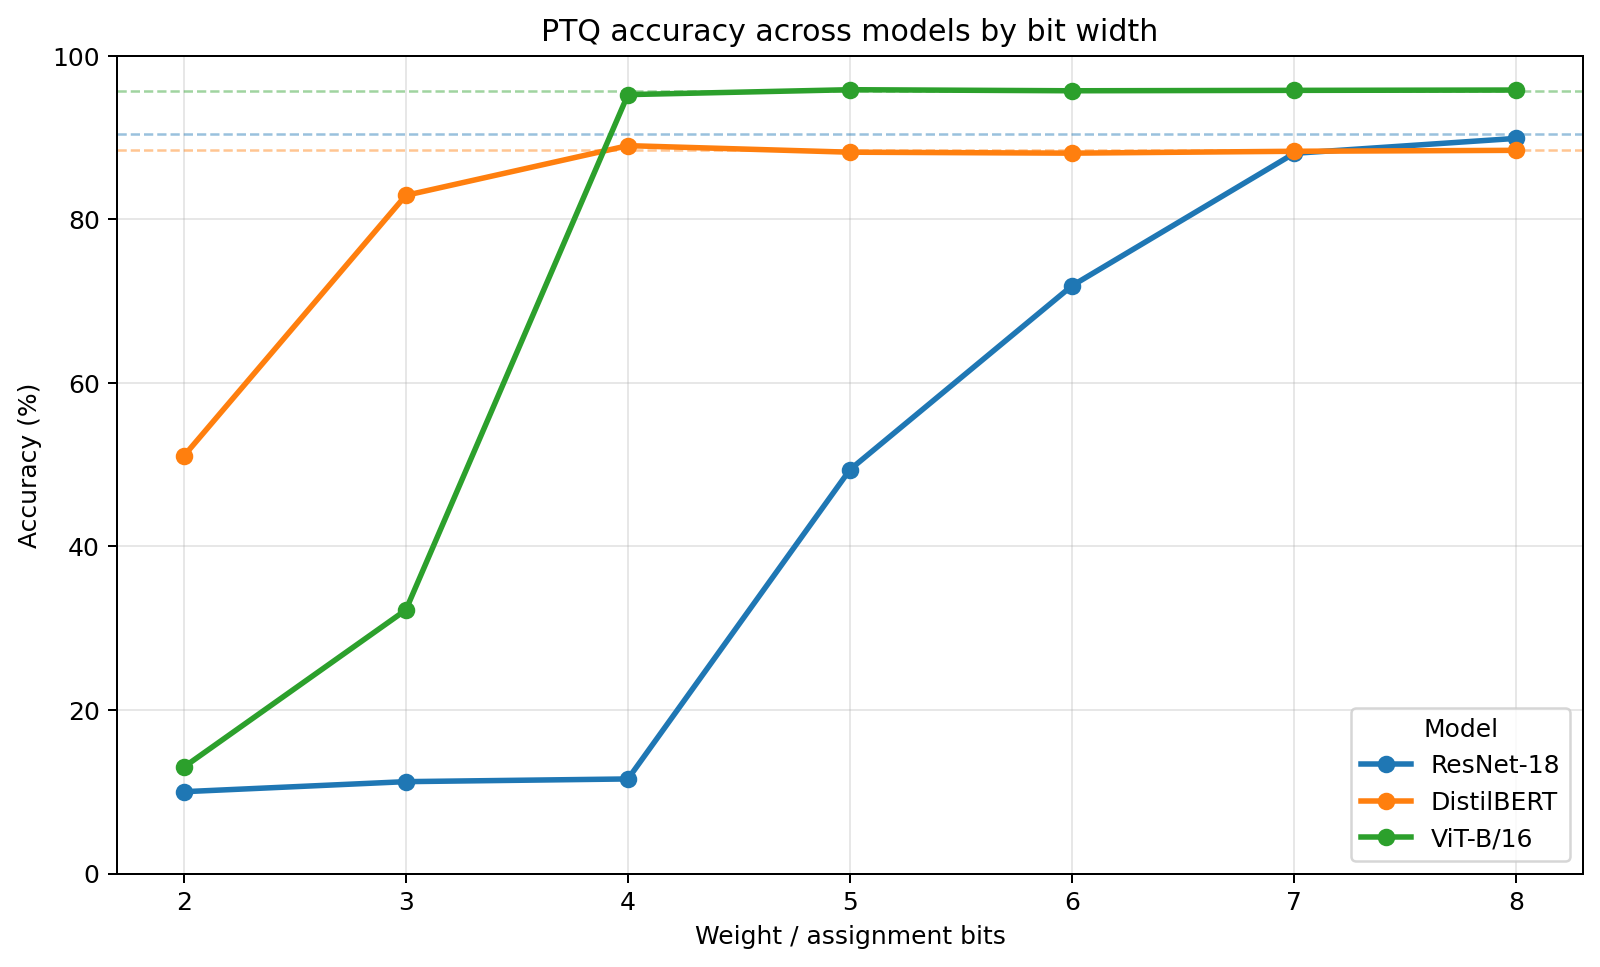
\includegraphics[width=.48\textwidth]{ptq_accuracy_all_models_2_to_8_bit.png}\hfill
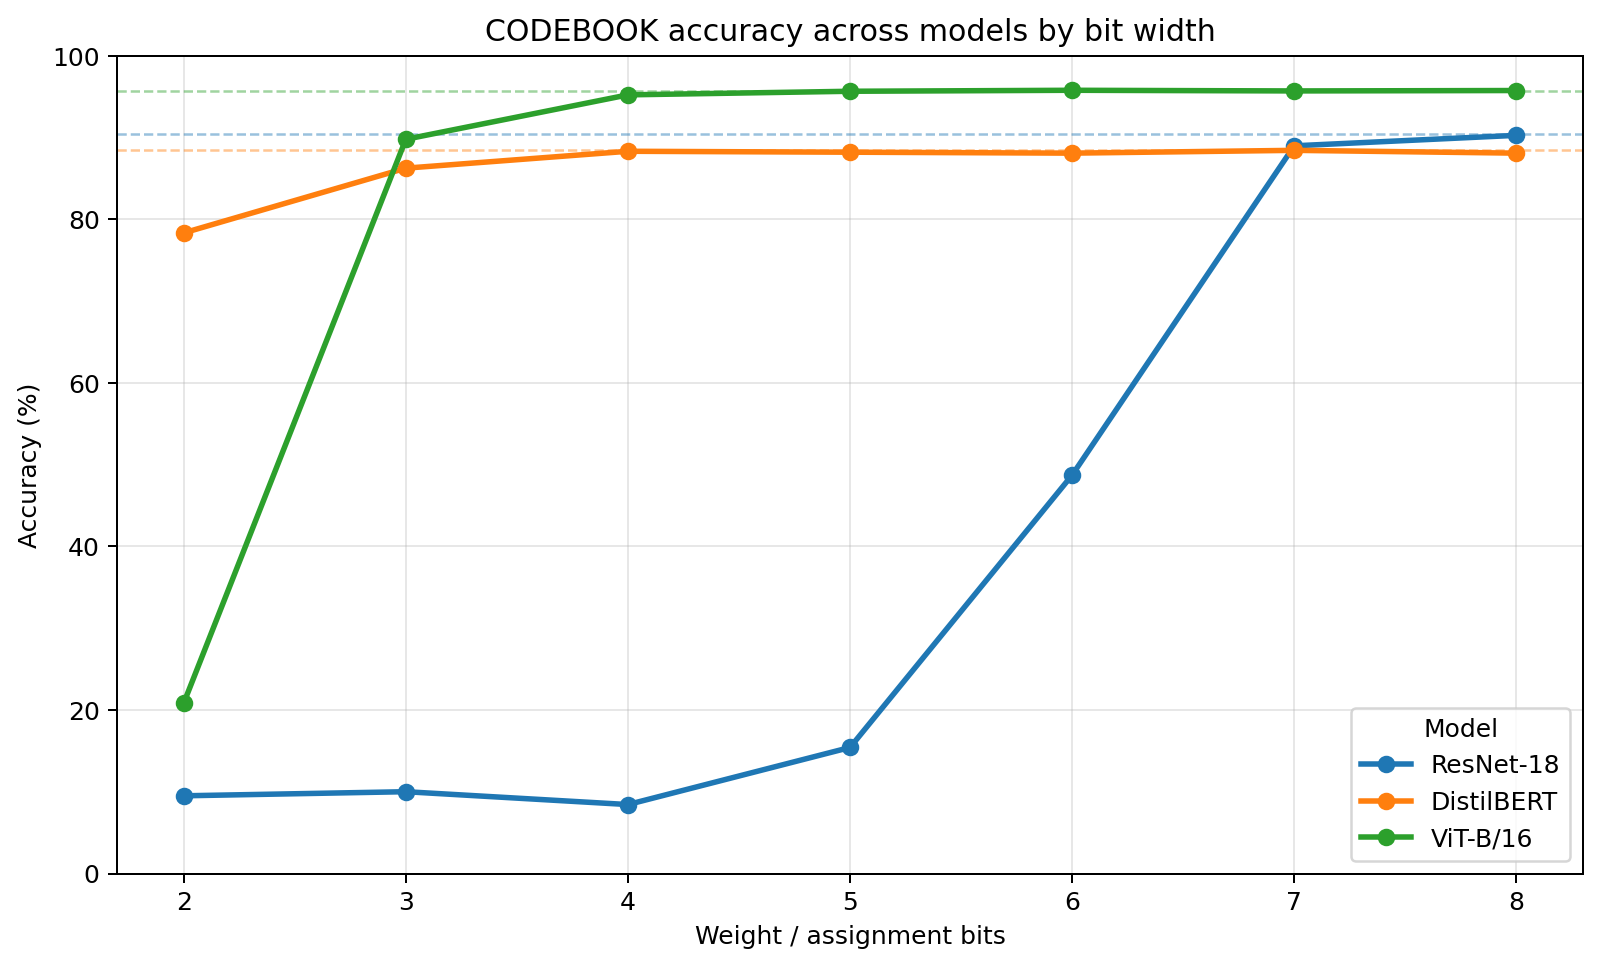
\includegraphics[width=.48\textwidth]{codebook_accuracy_all_models_2_to_8_bit.png}
\caption{Bit-wise accuracy across all three architectures for PTQ (left) and codebook quantization (right). Dashed lines show the corresponding FP32 baselines.}
\label{fig:cross-model-bitwise-accuracy}
\end{figure*}

ResNet-18 exhibits a severe low-bit transition under both methods (Table~\ref{tab:resnet-sweep}). PTQ remains near chance from two through four bits, then rises to 49.39\% at five bits, 71.87\% at six bits, and 88.05\% at seven bits. Codebook quantization recovers later: it reaches only 48.71\% at six bits but rises to 88.97\% at seven bits and 90.25\% at eight bits. Thus, W8 codebook is slightly closer to FP32 than W8 PTQ, but neither method makes full-model W4 ResNet usable.

\begin{table*}[t]
\caption{ResNet-18 PTQ and codebook sweep. $A$ is accuracy, $R$ is compression ratio, and $S$ is parameter-memory reduction.}
\label{tab:resnet-sweep}
\centering
\small
\begin{tabular}{@{}rrrrrrr@{}}
\toprule
Bits & PTQ $A$ & PTQ $R$ & PTQ $S$ & Codebook $A$ & Codebook $R$ & Codebook $S$ \\
\midrule
2 & 10.00\% & $15.60\times$ & 93.59\% & 9.50\% & $15.60\times$ & 93.59\% \\
3 & 11.23\% & $10.49\times$ & 90.47\% & 10.00\% & $10.49\times$ & 90.47\% \\
4 & 11.56\% & $7.91\times$ & 87.35\% & 8.43\% & $7.90\times$ & 87.35\% \\
5 & 49.39\% & $6.34\times$ & 84.23\% & 15.41\% & $6.34\times$ & 84.22\% \\
6 & 71.87\% & $5.29\times$ & 81.11\% & 48.71\% & $5.29\times$ & 81.10\% \\
7 & 88.05\% & $4.54\times$ & 77.99\% & 88.97\% & $4.54\times$ & 77.97\% \\
8 & 89.88\% & $3.98\times$ & 74.87\% & 90.25\% & $3.97\times$ & 74.82\% \\
\bottomrule
\end{tabular}
\end{table*}

DistilBERT behaves differently (Table~\ref{tab:distilbert-sweep}). At two bits, codebook quantization retains 78.33\% accuracy compared with 51.03\% for PTQ. At three bits, the gap narrows to 86.24\% versus 82.91\%. From four through eight bits, both methods remain within 0.58 percentage points of FP32.

\begin{table*}[t]
\caption{DistilBERT PTQ and codebook sweep. $A$ is accuracy, $R$ is compression ratio, and $S$ is parameter-memory reduction.}
\label{tab:distilbert-sweep}
\centering
\small
\begin{tabular}{@{}rrrrrrr@{}}
\toprule
Bits & PTQ $A$ & PTQ $R$ & PTQ $S$ & Codebook $A$ & Codebook $R$ & Codebook $S$ \\
\midrule
2 & 51.03\% & $15.67\times$ & 93.62\% & 78.33\% & $15.78\times$ & 93.66\% \\
3 & 82.91\% & $10.52\times$ & 90.49\% & 86.24\% & $10.57\times$ & 90.54\% \\
4 & 88.99\% & $7.92\times$ & 87.37\% & 88.30\% & $7.95\times$ & 87.42\% \\
5 & 88.19\% & $6.35\times$ & 84.25\% & 88.19\% & $6.37\times$ & 84.29\% \\
6 & 88.07\% & $5.30\times$ & 81.13\% & 88.07\% & $5.31\times$ & 81.17\% \\
7 & 88.30\% & $4.55\times$ & 78.01\% & 88.42\% & $4.55\times$ & 78.04\% \\
8 & 88.42\% & $3.98\times$ & 74.88\% & 88.07\% & $3.99\times$ & 74.92\% \\
\bottomrule
\end{tabular}
\end{table*}

The W4 PTQ result is 88.99\%, compared with the 88.42\% FP32 baseline: 776 rather than 771 correctly classified examples. This five-example difference is reported as an observed fluctuation on the small SST-2 development split and is not interpreted as evidence that quantization improves generalization.

ViT exhibits a stronger low-bit method interaction (Table~\ref{tab:vit-sweep}). At two bits, codebook accuracy is 20.84\% and PTQ accuracy is 13.00\%. At three bits, codebook quantization reaches 89.77\%, whereas PTQ reaches only 32.22\%. Both recover abruptly at four bits, reaching 95.20\% and 95.23\%, respectively. From four through eight bits, both methods remain close to the 95.73\% FP32 baseline.

\begin{table*}[t]
\caption{ViT-B/16 PTQ and codebook sweep. $A$ is accuracy, $R$ is compression ratio, and $S$ is parameter-memory reduction.}
\label{tab:vit-sweep}
\centering
\small
\begin{tabular}{@{}rrrrrrr@{}}
\toprule
Bits & PTQ $A$ & PTQ $R$ & PTQ $S$ & Codebook $A$ & Codebook $R$ & Codebook $S$ \\
\midrule
2 & 13.00\% & $15.50\times$ & 93.55\% & 20.84\% & $15.66\times$ & 93.62\% \\
3 & 32.22\% & $10.45\times$ & 90.43\% & 89.77\% & $10.52\times$ & 90.50\% \\
4 & 95.23\% & $7.88\times$ & 87.31\% & 95.20\% & $7.92\times$ & 87.37\% \\
5 & 95.83\% & $6.32\times$ & 84.19\% & 95.64\% & $6.35\times$ & 84.25\% \\
6 & 95.70\% & $5.28\times$ & 81.06\% & 95.76\% & $5.30\times$ & 81.13\% \\
7 & 95.75\% & $4.53\times$ & 77.94\% & 95.68\% & $4.55\times$ & 78.00\% \\
8 & 95.79\% & $3.97\times$ & 74.82\% & 95.73\% & $3.98\times$ & 74.87\% \\
\bottomrule
\end{tabular}
\end{table*}

Across the completed sweeps, compression is governed mainly by bit width because the selected tensors contain most model parameters. Two-bit representations provide approximately $15.5$--$15.8\times$ compression and about 93.6\% parameter-memory reduction. Four-bit representations provide approximately $7.9\times$ compression and about 87.3\% reduction. Eight-bit representations provide approximately $4\times$ compression and about 74.8--74.9\% reduction. Accuracy, unlike storage, remains strongly dependent on both architecture and quantization method.

Figure~\ref{fig:all-model-tradeoffs} consolidates accuracy, compression ratio, and parameter-memory reduction for all 42 configurations. The near-overlap of compression curves confirms that storage is determined primarily by bit width, whereas the separated accuracy curves expose architecture- and method-specific numerical sensitivity.

\begin{figure*}[!t]
\centering
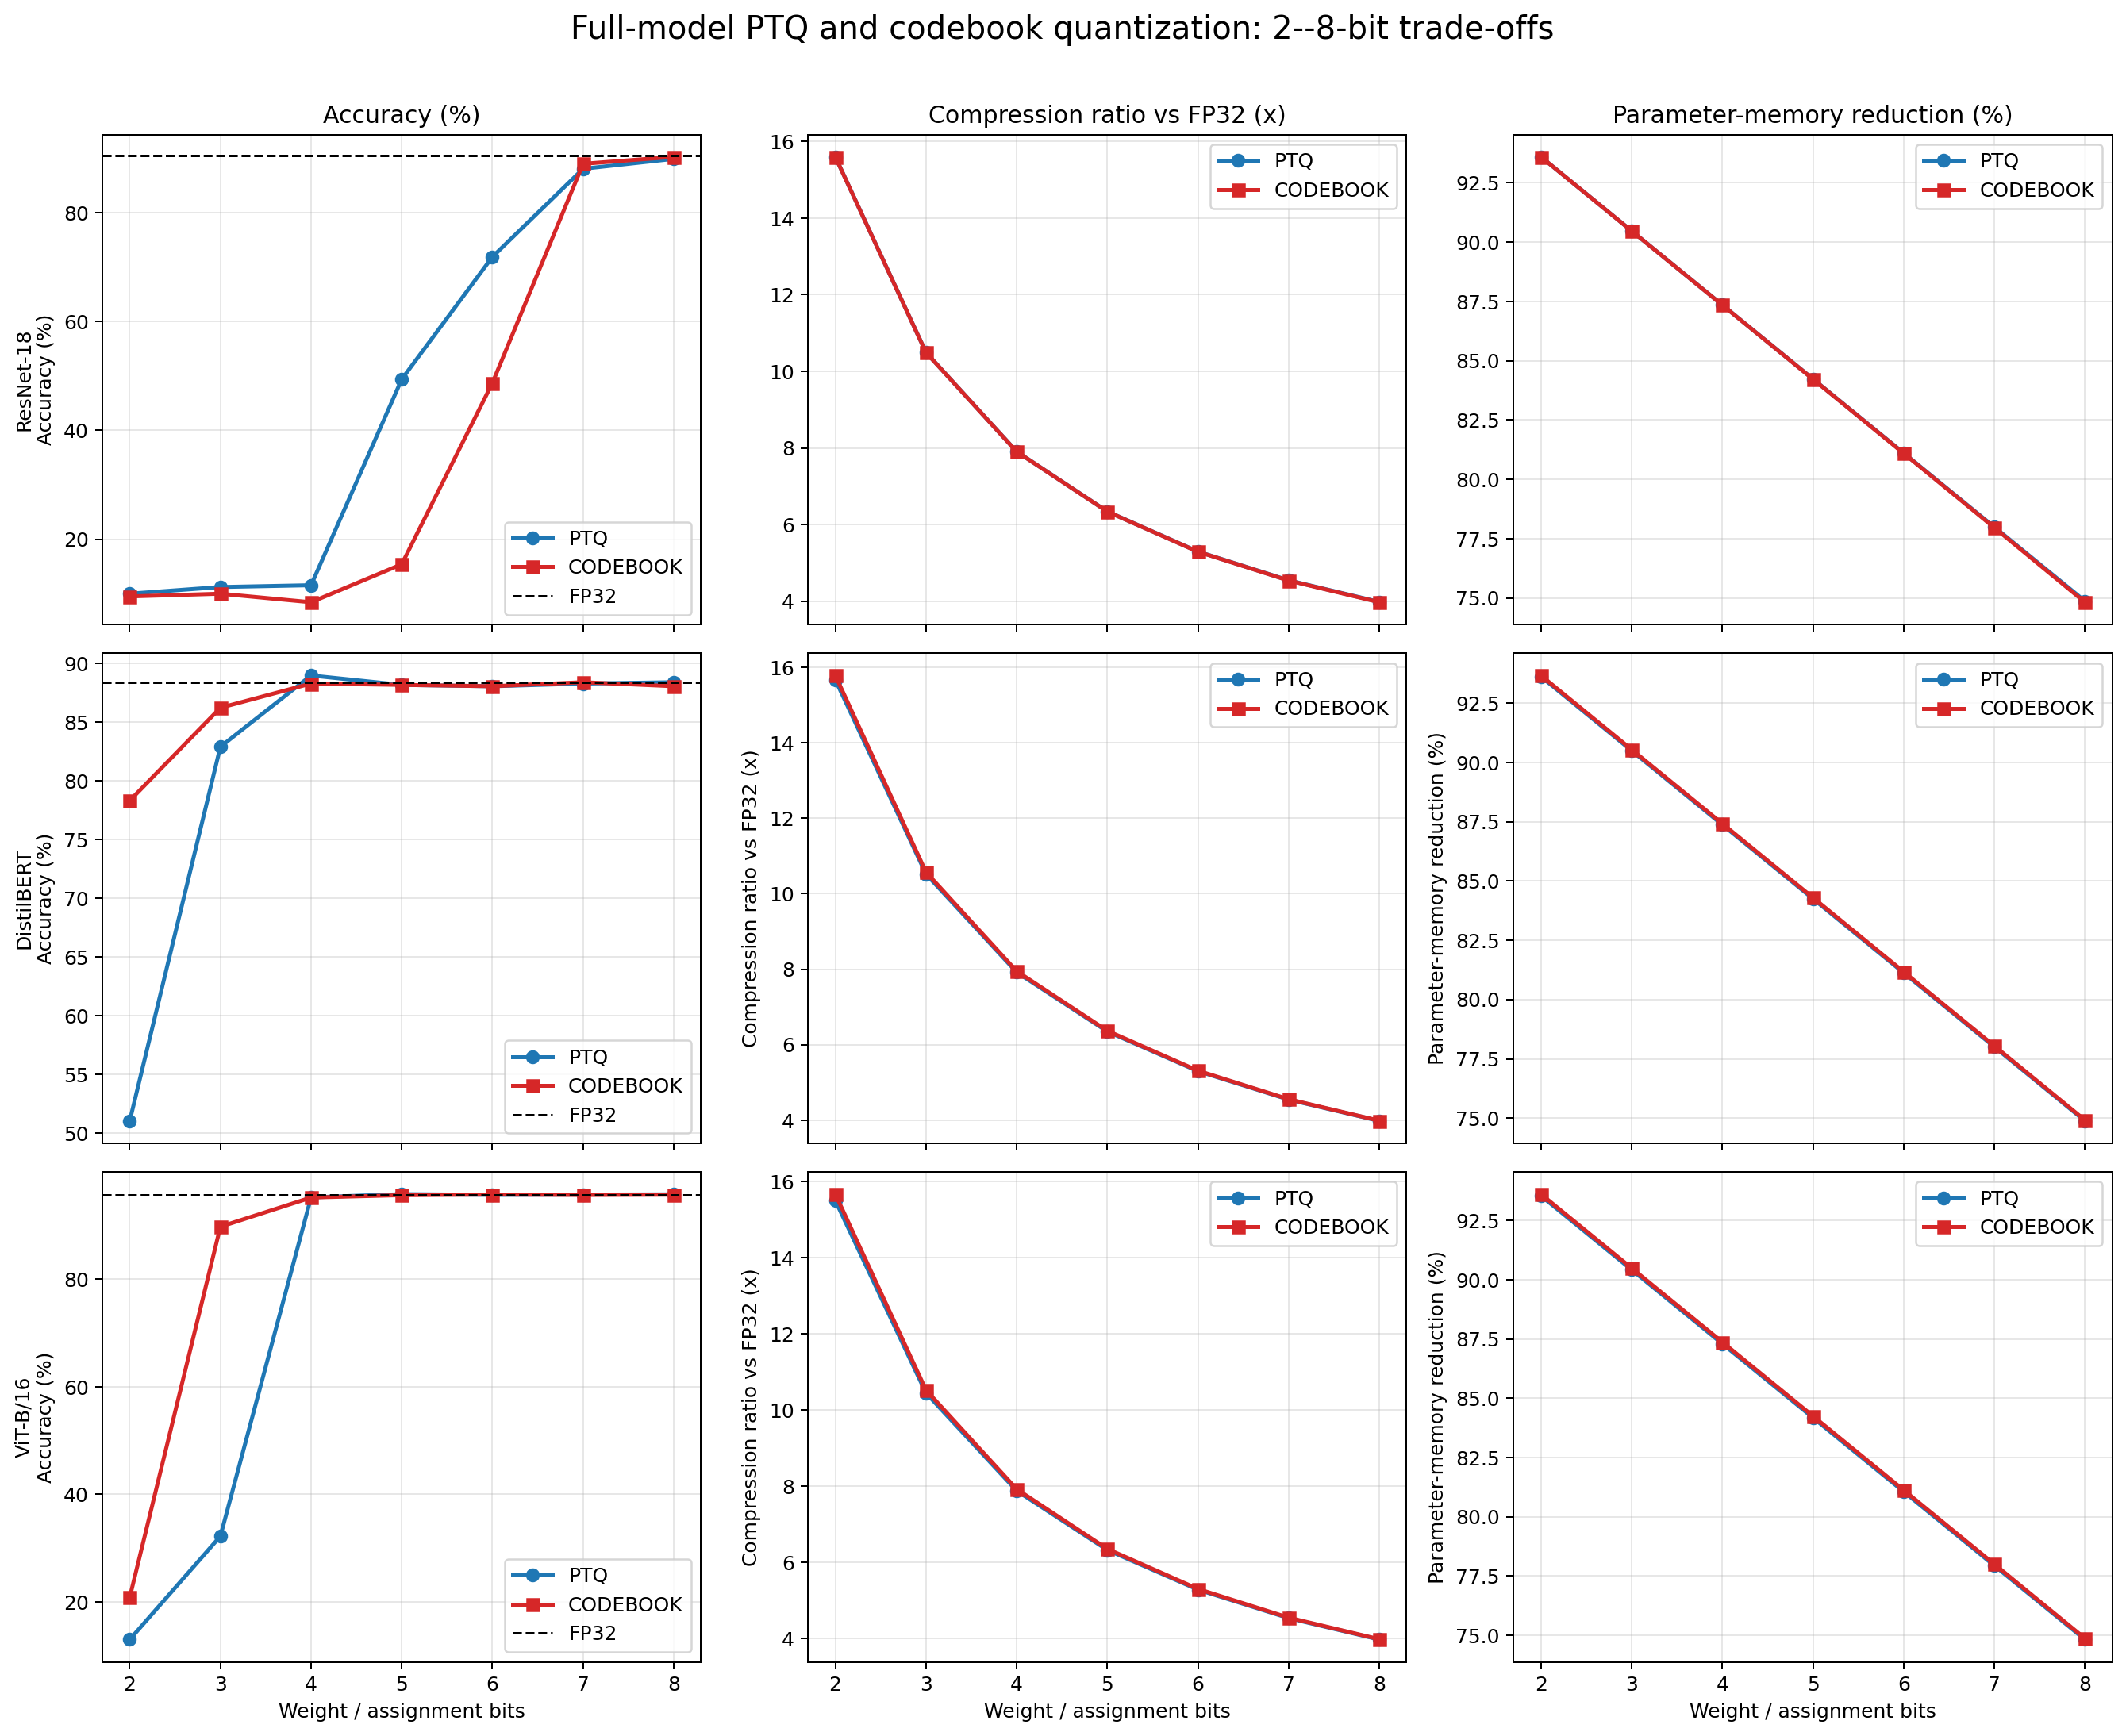
\includegraphics[width=.98\textwidth]{all_models_accuracy_compression_memory_2_to_8_bit.png}
\caption{Consolidated two-to-eight-bit results from Notebook~25. Rows correspond to ResNet-18, DistilBERT, and ViT-B/16; columns show accuracy, compression ratio, and parameter-memory reduction.}
\label{fig:all-model-tradeoffs}
\end{figure*}

\subsection{Layer and Module Sensitivity Analysis}
\label{sec:sensitivity}

\subsubsection{Motivation and experimental protocol}

The full-model sweeps identify when quantization fails, but they do not identify which internal components cause the failure. The sensitivity experiments therefore address two questions: which units are most sensitive, and whether a W8 sensitivity ranking transfers reliably to W4.

For an \emph{isolated sensitivity} run, the experiment starts from the original FP32 checkpoint, quantizes exactly one analysis unit, leaves every other parameter in FP32, and evaluates the resulting model on the complete labelled evaluation split. ResNet uses individual eligible kernels, DistilBERT uses individual eligible embedding or kernel tensors, and ViT groups its 76 eligible tensors into 14 logical modules. Accuracy degradation is
\begin{equation}
\Delta A_u=A_{\mathrm{FP32}}-A_u,
\end{equation}
where $A_u$ is the accuracy when only unit $u$ is quantized. A negative value means that the configuration happens to classify more evaluation examples correctly; it is not treated as evidence of improved generalization.

Table~\ref{tab:sensitivity-coverage} summarizes the analysis coverage. All configurations use the complete evaluation split. ResNet is exhaustive at both precisions. DistilBERT and ViT are exhaustive at W8, but their W4 isolated studies use predefined architecture-stratified subsets to make the long-running experiments feasible. The subsets were fixed before inspecting W4 outcomes.

\subsubsection{Isolated W8 and W4 sensitivity}

Table~\ref{tab:isolated-sensitivity-summary} reports the largest isolated accuracy loss for every architecture, method, and precision. At W8, all three architectures are stable: the largest isolated loss is only 0.53\pp. At W4, the transformer results remain small over their stratified samples, whereas ResNet becomes highly non-uniform. Quantizing only its first convolution reduces accuracy by 60.65\pp under PTQ and 78.62\pp under codebook quantization. Thirteen of 21 W4 codebook kernels and 14 of 21 W4 PTQ kernels remain significant after false-discovery-rate correction. No sampled DistilBERT or ViT unit is FDR-significant.

Figure~\ref{fig:resnet-cross-bit-sensitivity} visualizes the ResNet result. W8 perturbations are small across all kernels, while W4 exposes a small set of severe early-layer failures. This provides a component-level explanation for the full-model W4 collapse observed in Table~\ref{tab:resnet-sweep}.

\subsubsection{Cross-bit rank stability}

The next experiment tests whether the W8 sensitivity order predicts behavior at W4. Spearman rank correlations are calculated over matched units. Table~\ref{tab:cross-bit-rank-stability} shows that rank transfer is generally unreliable. ResNet and ViT correlations are negative and non-significant, and DistilBERT PTQ is also non-significant. DistilBERT codebook quantization is the only tested case with a statistically significant positive relationship ($\rho=0.693$, $p=0.004$). Consequently, W8 sensitivity should not be assumed to identify W4-sensitive components without validation.

\begin{table}[!t]
\centering
\caption{Coverage of the isolated sensitivity experiments. ``Strat.'' denotes a predefined architecture-stratified W4 subset.}
\label{tab:sensitivity-coverage}
\scriptsize
\setlength{\tabcolsep}{2.5pt}
\begin{tabular}{@{}llllr@{}}
\toprule
Model & Unit & W8 & W4 & Examples \\
\midrule
ResNet-18 & Kernel & 21/21 & 21/21 & 10,000 \\
DistilBERT & Tensor & 40/40 & 15/40 (strat.) & 872 \\
ViT-B/16 & Module & 14/14 & 7/14 (strat.) & 10,000 \\
\bottomrule
\end{tabular}
\end{table}

\begin{table}[!t]
\centering
\caption{Maximum isolated accuracy degradation. Transformer W4 values refer to predefined stratified samples; ``Sig.'' gives the FDR-significant count.}
\label{tab:isolated-sensitivity-summary}
\scriptsize
\setlength{\tabcolsep}{2pt}
\begin{tabular}{@{}llrrlr@{}}
\toprule
Model & Method & Bits & Drop (pp) & Most sensitive unit & Sig. \\
\midrule
ResNet-18 & PTQ & 8 & 0.53 & First convolution & 1/21 \\
ResNet-18 & Codebook & 8 & 0.52 & First convolution & 1/21 \\
ResNet-18 & PTQ & 4 & 60.65 & First convolution & 14/21 \\
ResNet-18 & Codebook & 4 & 78.62 & First convolution & 13/21 \\
\midrule
DistilBERT & PTQ & 8 & 0.115 & L1 attention value & 0/40 \\
DistilBERT & Codebook & 8 & 0.229 & L2 intermediate FFN & 0/40 \\
DistilBERT & PTQ & 4 & 0.115 & L2 intermediate FFN & 0/15 \\
DistilBERT & Codebook & 4 & 0.229 & L2 intermediate FFN & 0/15 \\
\midrule
ViT-B/16 & PTQ & 8 & 0.02 & Transformer block 4 & 0/14 \\
ViT-B/16 & Codebook & 8 & 0.06 & Transformer block 6 & 0/14 \\
ViT-B/16 & PTQ & 4 & 0.04 & Transformer block 6 & 0/7 \\
ViT-B/16 & Codebook & 4 & 0.20 & Transformer block 1 & 0/7 \\
\bottomrule
\end{tabular}
\end{table}

\begin{figure}[!t]
\centering
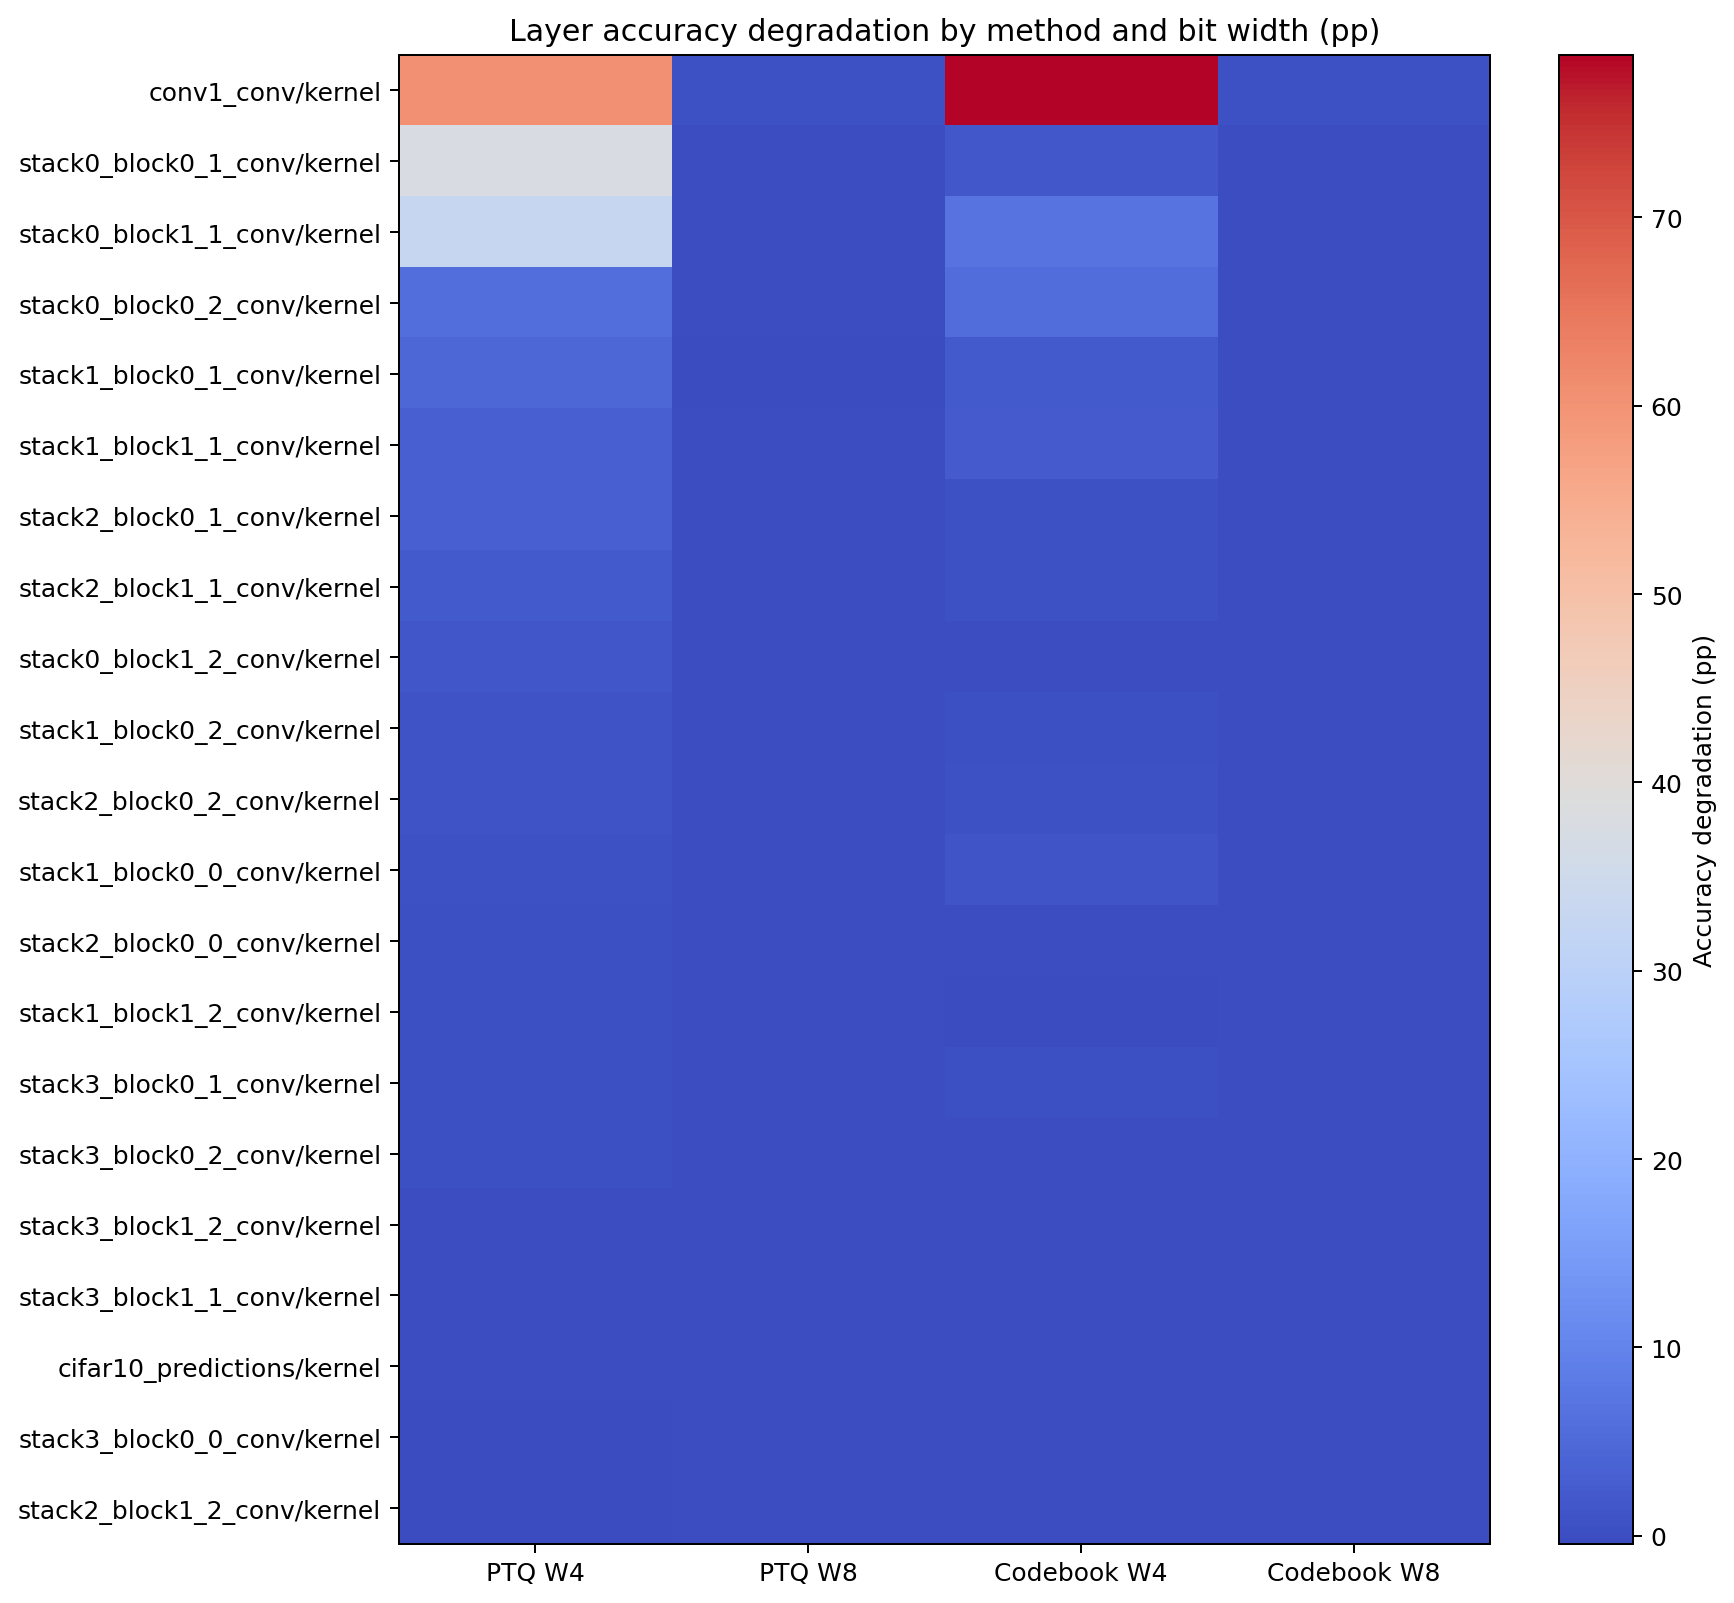
\includegraphics[width=\columnwidth]{resnet18_w4_w8_layer_sensitivity.png}
\caption{Matched ResNet-18 isolated kernel sensitivity at W4 and W8 for PTQ and codebook quantization. Only one kernel is quantized in each evaluation.}
\label{fig:resnet-cross-bit-sensitivity}
\end{figure}

\begin{table}[!t]
\centering
\caption{W4/W8 sensitivity-rank stability}
\label{tab:cross-bit-rank-stability}
\small
\begin{tabular}{@{}llrr@{}}
\toprule
Model & Method & Spearman $\rho$ & $p$-value \\
\midrule
ResNet-18 & PTQ & $-0.094$ & 0.687 \\
ResNet-18 & Codebook & $-0.292$ & 0.199 \\
DistilBERT & PTQ & 0.143 & 0.612 \\
DistilBERT & Codebook & 0.693 & 0.004 \\
ViT-B/16 & PTQ & $-0.321$ & 0.482 \\
ViT-B/16 & Codebook & $-0.357$ & 0.432 \\
\bottomrule
\end{tabular}
\end{table}

\FloatBarrier

\section{Limitations}

Statistical significance for isolated sensitivity experiments was assessed using paired McNemar tests \cite{dietterich1998}, followed by Benjamini--Hochberg false-discovery-rate correction across the tested units \cite{benjamini1995}. Spearman rank correlation was used to compare W4 and W8 sensitivity rankings.

Three limitations qualify the conclusions. First, the DistilBERT and ViT W4 isolated studies cover predefined architecture-stratified subsets rather than all eligible units. Second, DistilBERT is evaluated on the relatively small labelled SST-2 development split, so changes of one or two examples produce visible accuracy differences. Third, the custom models reconstruct quantized weights for FP32 Keras execution. The storage results therefore describe parameter representations and do not demonstrate latency, energy, throughput, or runtime-memory improvements.

\section{Conclusion}

This study analyzed uniform per-channel PTQ and non-uniform codebook weight quantization in two transformer architectures, using ResNet-18 as a CNN reference. Across all three models, W8 preserved accuracy while reducing estimated parameter storage by approximately 75\%. The central architecture-level result appears at W4: DistilBERT and ViT-B/16 remained within 0.6 percentage points of their FP32 baselines at about $7.9\times$ compression, whereas ResNet-18 collapsed to near-chance accuracy under both methods.

The low-bit sweeps also show that the quantization method matters most below four bits. Codebook quantization substantially outperformed PTQ for DistilBERT at W2 and for ViT at W3, but neither method provided uniformly reliable performance at the lowest precisions. A plausible, untested explanation for the 57.55-percentage-point ViT W3 gap is that learned codebook centroids adapt to a non-uniform weight distribution, whereas a three-bit uniform PTQ grid provides too few fixed levels to represent the same weights adequately. The isolated sensitivity analysis explains part of the CNN failure: ResNet's first convolution was exceptionally vulnerable at W4, while the sampled transformer tensors and modules produced much smaller isolated losses. Cross-bit rank correlations were generally weak, so sensitivity observed at W8 should not be treated as a dependable proxy for W4 behavior.

Overall, the evaluated transformer models are more tolerant of four-bit weight quantization than the CNN reference under the stated selection and evaluation policies. This makes low-bit transformer storage promising, but the conclusion is limited to model accuracy and parameter representation. Future deployment work should execute genuinely packed low-bit kernels and measure latency, runtime memory, throughput, and energy on target hardware before claiming computational-efficiency gains.

\FloatBarrier

\IEEEtriggeratref{12}
\begin{thebibliography}{99}

\bibitem{jacob2018}
B. Jacob et al., ``Quantization and training of neural networks for efficient integer-arithmetic-only inference,'' in \emph{Proc. IEEE/CVF Conf. Computer Vision and Pattern Recognition (CVPR)}, 2018, pp. 2704--2713.

\bibitem{krishnamoorthi2018}
R. Krishnamoorthi, ``Quantizing deep convolutional networks for efficient inference: A whitepaper,'' arXiv:1806.08342, 2018.

\bibitem{nagel2021}
M. Nagel et al., ``A white paper on neural network quantization,'' arXiv:2106.08295, 2021.

\bibitem{vaswani2017}
A. Vaswani et al., ``Attention is all you need,'' in \emph{Proc. Advances in Neural Information Processing Systems (NeurIPS)}, vol.~30, 2017.

\bibitem{gray1984}
R. M. Gray, ``Vector quantization,'' \emph{IEEE ASSP Magazine}, vol. 1, no. 2, pp. 4--29, 1984.

\bibitem{arthur2007}
D. Arthur and S. Vassilvitskii, ``k-means{+}{+}: The advantages of careful seeding,'' in \emph{Proc. 18th Annual ACM-SIAM Symp. Discrete Algorithms (SODA)}, 2007, pp.~1027--1035.

\bibitem{lloyd1982}
S.~P. Lloyd, ``Least squares quantization in PCM,'' \emph{IEEE Trans. Information Theory}, vol.~28, no.~2, pp.~129--137, 1982.

\bibitem{jegou2011}
H. J\'egou, M. Douze, and C. Schmid, ``Product quantization for nearest neighbor search,'' \emph{IEEE Trans. Pattern Analysis and Machine Intelligence}, vol. 33, no. 1, pp. 117--128, 2011.

\bibitem{gong2014}
Y. Gong, L. Liu, M. Yang, and L. Bourdev, ``Compressing deep convolutional networks using vector quantization,'' arXiv:1412.6115, 2014.

\bibitem{han2016}
S. Han, H. Mao, and W. J. Dally, ``Deep compression: Compressing deep neural networks with pruning, trained quantization and Huffman coding,'' in \emph{Proc. International Conf. Learning Representations (ICLR)}, 2016.

\bibitem{choi2017}
J. Choi, Z. Wang, S. Venkataramani, P. I.-J. Chuang, V. Srinivasan, and K. Gopalakrishnan, ``Towards the limit of network quantization,'' in \emph{Proc. ICLR Workshop on Efficient Methods for Deep Neural Networks}, 2017.

\bibitem{shao2024}
J. Shao, H. Zhang, and J. Wu, ``Diffusion product quantization,'' arXiv:2411.12306, 2024.

\bibitem{deng2024}
J. Deng, S. Li, Z. Wang, H. Gu, K. Xu, and K. Huang, ``VQ4ALL: Efficient neural network representation via a universal codebook,'' arXiv:2412.06875, 2024.

\bibitem{abushahla2025}
H. A. Abushahla, D. Varam, A. J. N. Panopio, and M. I. AlHajri, ``Quantized neural networks for microcontrollers: A comprehensive review of methods, platforms, and applications,'' arXiv:2508.15008, 2025.

\bibitem{he2016}
K. He, X. Zhang, S. Ren, and J. Sun, ``Deep residual learning for image recognition,'' in \emph{Proc. IEEE Conf. Computer Vision and Pattern Recognition (CVPR)}, 2016, pp. 770--778.

\bibitem{krizhevsky2009}
A. Krizhevsky, ``Learning multiple layers of features from tiny images,'' University of Toronto, Toronto, Canada, Tech. Rep., 2009.

\bibitem{sanh2019}
V. Sanh, L. Debut, J. Chaumond, and T. Wolf, ``DistilBERT, a distilled version of BERT: Smaller, faster, cheaper and lighter,'' arXiv:1910.01108, 2019.

\bibitem{socher2013}
R. Socher et al., ``Recursive deep models for semantic compositionality over a sentiment treebank,'' in \emph{Proc. Conf. Empirical Methods in Natural Language Processing (EMNLP)}, 2013, pp. 1631--1642.

\bibitem{wang2018}
A. Wang et al., ``GLUE: A multi-task benchmark and analysis platform for natural language understanding,'' in \emph{Proc. International Conf. Learning Representations (ICLR)}, 2019.

\bibitem{dosovitskiy2021}
A. Dosovitskiy et al., ``An image is worth 16x16 words: Transformers for image recognition at scale,'' in \emph{Proc. International Conf. Learning Representations (ICLR)}, 2021.

\bibitem{dietterich1998}
T.~G. Dietterich, ``Approximate statistical tests for comparing supervised classification learning algorithms,'' \emph{Neural Computation}, vol.~10, no.~7, pp.~1895--1923, 1998.

\bibitem{benjamini1995}
Y. Benjamini and Y. Hochberg, ``Controlling the false discovery rate: A practical and powerful approach to multiple testing,'' \emph{J. Royal Statistical Society B}, vol.~57, no.~1, pp.~289--300, 1995.

\end{thebibliography}

\end{document}
